\chapter{Fashion Entrepreneurs Wise Life Advice}

This lecture is brief, but it is not loose. It begins with a backward-looking question and answers it with two ranked lessons: first, relationships matter most; second, customer service makes people return and speak well of us. There are no validated board figures or equations to preserve here, so the mathematics in what follows is deliberately light and explicitly reconstructive. Its purpose is only to make the speaker's commercial mechanism visible while keeping the transcript's order, emphasis, and payoff.

\begin{remark}
The formulas in this chapter are not quoted from a board. They are compact notational summaries of the lecture's causal claims, introduced only where they help us keep the argument in view.
\end{remark}

\section{The Retrospective Setup}

The opening question gives the whole lecture its shape: if we could go back to the beginning of the business, what are the two things we would most want to have known? That is already a strong discipline. We are not collecting general advice; we are isolating the two missing pieces that, in hindsight, would have changed the early trajectory of the business.

The answer comes in order. The speaker does not wander. He gives a first principle, then an example that shows why it matters, then a second principle, then a comparison that sharpens it, and finally a closing imperative. The chapter should preserve that unfolding rather than flatten it into a list of slogans.

\section{First Lesson: Relationships Before Technique}

The first lesson is stated almost as a ranking principle: relationships are the most important thing in the world. Immediately after that comes the compressed business proverb, ``it is not what you know, it is who you know.'' We can preserve that compression by introducing
\[
R = \text{relationship capital},
\qquad
O = \text{downstream opportunity}.
\]
Then the first lesson takes the compact form
\begin{equation}
R \to O.
\end{equation}

This arrow is not a theorem in the strict sense. It is a directional claim about how motion often occurs in a commercial world. Access, invitations, referrals, and introductions do not always come from formal procedure; they often come through persons who remember us, trust us, and are willing to connect us to the next room.

If we want a second summary line, we may write
\begin{equation}
O \propto R,
\end{equation}
but we should read it modestly. The lecture is not proposing a measurable law. It is saying only that a richer stock of trusted relationships tends, other things equal, to enlarge the field of available opportunity.

\section{Evidence: From Service to Opportunity}

The speaker does not leave the proverb suspended in the air. He supplies a concrete example: he says that he has judged three fashion shows in the past year because of a relationship that grew out of giving great customer service to someone else. The transcript is slightly garbled at this point, so we should paraphrase cautiously, but the mechanism is sufficiently clear.

Let
\[
S = \text{service quality},
\qquad
T = \text{remembered trust}.
\]
Then the anecdote suggests the chain
\begin{align}
S &\to T,\\
T &\to R,\\
R &\to O.
\end{align}
Putting the steps together, we obtain the lecture's implied pathway:
\begin{equation}
S \to T \to R \to O.
\end{equation}

This is the first moment at which the lecture becomes more than a slogan. A good interaction is not exhausted when the transaction ends. It can leave a residue; that residue can become trust; trust can stabilize into relationship; and relationship can later return in a different commercial form from the original service event.

The count matters here. The speaker does not say merely that something good happened later. He says that he judged three fashion shows. That number should remain in the notes because it is the one explicit quantitative marker in the interview, and it gives the anecdote commercial weight.

\subsection{Question \& Answer}

\paragraph{Question.} How can one act of customer service to one person later reappear as an opportunity in a different setting?

\paragraph{Answer.} Because the first act is not commercially terminal. It creates a memory. If that memory is favorable and durable, it becomes trust; if trust is attached to a person rather than to an abstract brand image, it becomes relationship capital; and relationship capital can later be cashed out as access.

The logic can be written as a short derivation.

\begin{enumerate}
\item A strong service interaction produces a positive remembered impression.
\item A remembered impression, if it persists, becomes trust rather than mere recollection.
\item Trust attached to a person contributes to relationship capital.
\item Relationship capital can later be converted into invitations, referrals, or access.
\end{enumerate}

The important point is not that every good interaction will produce a dramatic later reward. The point is the direction of the mechanism: the sale is over, but the commercial effect may not be over.

\section{Secondly: Customer Service Makes People Come Back}

At this point the lecture makes its hinge explicit: ``Secondly.'' The speaker even emphasizes the plainness of the point, saying that he cannot explain it more than this. Customer service makes people come back, and word of mouth advertising is the best.

We therefore introduce
\[
B = \text{return business},
\qquad
W = \text{word-of-mouth effect}.
\]
Then the second lesson is
\begin{equation}
S \to B \to W.
\end{equation}

This is a useful pivot because it connects the second lesson back to the first. If relationships create opportunity, customer service is one of the main ways by which relationships are first formed and then reinforced. The lecture does not present these as two unrelated virtues. They are two views of the same commercial sequence.

Notice also the order of emphasis. The speaker first says that customer service brings people back. Only then does he add that word of mouth is the best advertising. Return business comes first in the sequence, public reputation second. The notes should preserve that temporal order.

\section{Word of Mouth Versus Scripted Courtesy}

Now the speaker sharpens the second lesson by way of comparison. He asks us to think about entering a Walmart or a Dollar Tree. We hear the greeting; yet, because it has been repeated so many times, it no longer feels personal. This is not a rejection of politeness. It is a distinction between a script and a relation.

To keep that distinction visible, let
\[
A = \text{authenticity or personal quality of service}.
\]
Then the closing practical rule of this section may be summarized as
\begin{equation}
A \uparrow \;\Rightarrow\; W \uparrow.
\end{equation}
Again, the notation is qualitative. It says only that as the interaction becomes more genuinely personal, it becomes more likely to circulate in speech and memory.

We can make the comparison slightly more explicit by using a toy update rule. Let \(A_n \in \{0,1\}\) record the quality of the \(n\)-th encounter, with \(A_n = 0\) for scripted courtesy and \(A_n = 1\) for personal service. Then a minimal bookkeeping model is
\begin{align}
B_{n+1} &= B_n + \phi(A_n),\\
W_{n+1} &= W_n + \psi(B_{n+1}),
\end{align}
where \(\phi(1) > \phi(0)\) and \(\psi\) is increasing. We should not mistake this for a measured retail model. It is simply a compact way to preserve the lecture's point that not all customer contact is commercially equal.

Because no validated screenshot evidence survived review for this lecture, the diagram below is not a transcription of a visible board. It is a synthesis diagram, included only to keep the two spoken mechanisms in one field of view.

\begin{figure}[h]
\centering
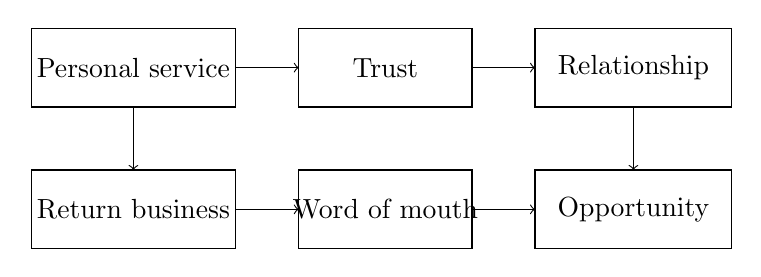
\begin{tikzpicture}[x=1cm,y=1cm]
\draw (0,0) rectangle (2.6,1) node[pos=.5]{Personal service};
\draw[->] (2.6,0.5) -- (3.4,0.5);
\draw (3.4,0) rectangle (5.6,1) node[pos=.5]{Trust};
\draw[->] (5.6,0.5) -- (6.4,0.5);
\draw (6.4,0) rectangle (8.9,1) node[pos=.5]{Relationship};

\draw[->] (1.3,0) -- (1.3,-0.8);
\draw (0,-1.8) rectangle (2.6,-0.8) node[pos=.5]{Return business};
\draw[->] (2.6,-1.3) -- (3.4,-1.3);
\draw (3.4,-1.8) rectangle (5.6,-0.8) node[pos=.5]{Word of mouth};
\draw[->] (5.6,-1.3) -- (6.4,-1.3);
\draw (6.4,-1.8) rectangle (8.9,-0.8) node[pos=.5]{Opportunity};

\draw[->] (7.65,0) -- (7.65,-0.8);
\end{tikzpicture}
\end{figure}

The upper row tells us how service can become relationship. The lower row tells us how service can become repeat trade and public reputation. The vertical arrow on the right closes the thought back to the speaker's anecdote: relationships do not merely feel good; they open doors.

\section{Make It Personal}

The lecture ends with a command rather than a summary sentence: make it personal. That is the right ending, because it binds the two earlier lessons into one operational rule.

If the interaction is generic, it may finish the transaction but leave very little behind. If it is personal, it leaves a trace. That trace may become trust; trust may become relationship; relationship may create opportunity; and personal treatment may also bring customers back and prompt them to speak well of us. What looked at first like two pieces of advice is therefore really one mechanism viewed from two sides.

The first side is external: relationships create access. The second side is generative: customer service is one of the ways by which those relationships are made and remembered. The lecture's closing imperative is therefore not sentimental. It is a disciplined piece of commercial reasoning.

\section{Summary}

The chapter can be compressed into three linked causal lines:
\[
R \to O,
\qquad
S \to B \to W,
\qquad
S \to T \to R \to O.
\]
The first says that relationships generate opportunity. The second says that customer service generates return business and word of mouth. The third says that the deeper bridge between them is remembered trust.

In that form the interview becomes more than a collection of aphorisms. It becomes a small, careful theory of business aftereffects. What we do in one encounter may continue to act after the encounter is over. That is why the lecture ends where it does: if we want the market to remember us, we must make the interaction personal.